\section{Architecture 103}

\subsection{Preliminary concept}

\textbf{State - Stateful - Stateless}

\begin{itemize}
	\item State
	variable and instances of a system at a given time
	\item Stateful
	capability of a system to remember preceding event or user insteraction
	e.g., an applicative session of an authenticated user on a Web Site
	\item Stateless
	capability of a system to response always in the same way independently to any sort of previus state
	e.g., a REST API
\end{itemize}

\textbf{Table index*}

\begin{itemize}
	\item An index is an optional structure, associated with a table or table cluster, that sometimes speed data access
	\item By creating an index on one or more caloumns of a table, you gian the ability in some cases to retrive a small set of randomly distributed rows from the table
\end{itemize}

\textbf{Long story short - Lesson Index}

Today we will focus on 3 possibile design patterns
\begin{itemize}
	\item Where and Diff - Change data capture
	How to incrementally retrive data in Big Data and Legacy Apps
	\item Move and Rename - Stateless change data capture
	How not to start from beginning
	\item Wrapper - Lock-in free solutions
	How to mitigate vendor lock-in
\end{itemize}

\subsection{Data Source}

\subsubsection{Data Sources - Log Data}

\begin{center}
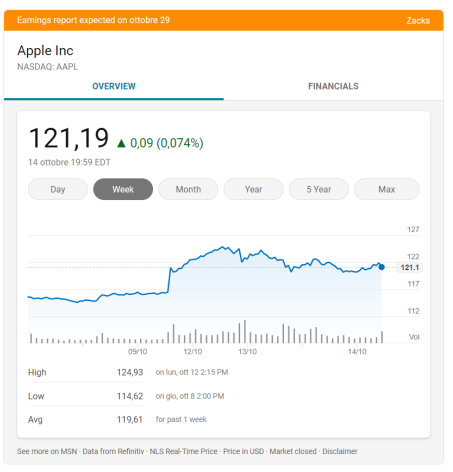
\includegraphics[scale=0.5]{24-data-source-log-data-1}
\end{center}

\begin{itemize}
	\item A log data table is a table that \textbf{records events}
	\item Because of the past cannot be undone, a log table allow INSERT only transactions
	\item E.g., buy/sell transactions of a company in Stock Market
\end{itemize}

Solution: Remeber the \textbf{last timestamp}

\hrulefill

\begin{center}
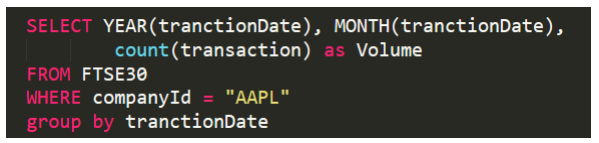
\includegraphics[scale=0.5]{25-data-source-log-data-2}
\end{center}

\begin{center}
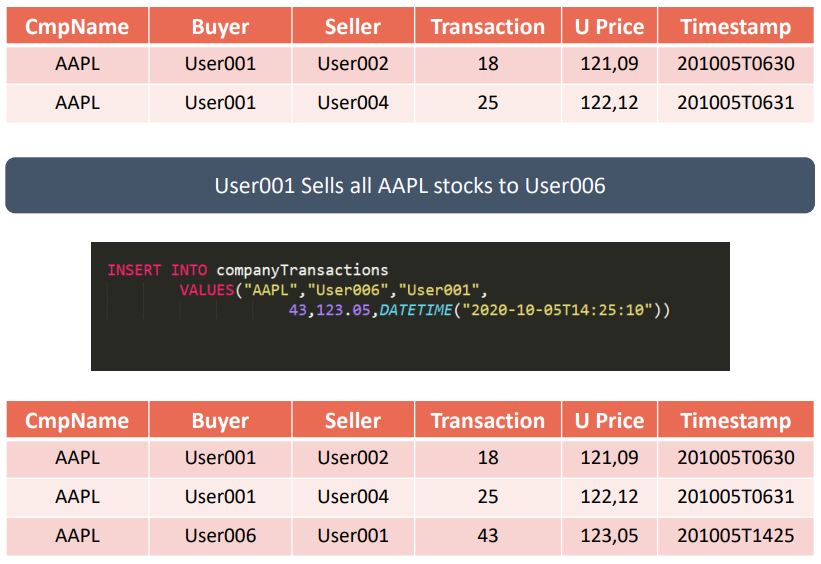
\includegraphics[scale=0.5]{26-data-source-log-data-3}
\end{center}

\hrulefill

\subsubsection{Data Sources – Registry Data (a.k.a. Master Data Table)}

\begin{center}
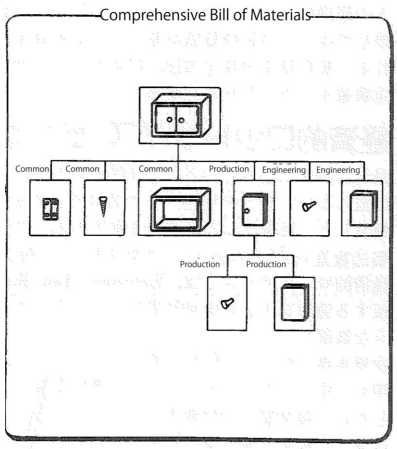
\includegraphics[scale=0.5]{27-data-source-registry-data-1}
\end{center}

\begin{itemize}
	\item A Registry Data Table describe \textbf{entities could change} over
time
	\item Because of this nature, all the 4 main verbs (SELECT,
INSERT, UPDATE, DELETE) can be used on it
	\item E.g., the full list of material needed to produce something
– called Bill of Material (BOM)
\end{itemize}

\begin{center}
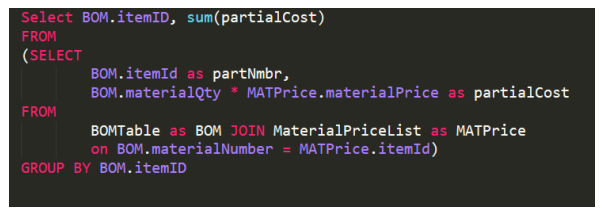
\includegraphics[scale=0.5]{28-data-source-registry-data-2}
\end{center}

\hrulefill

\begin{center}
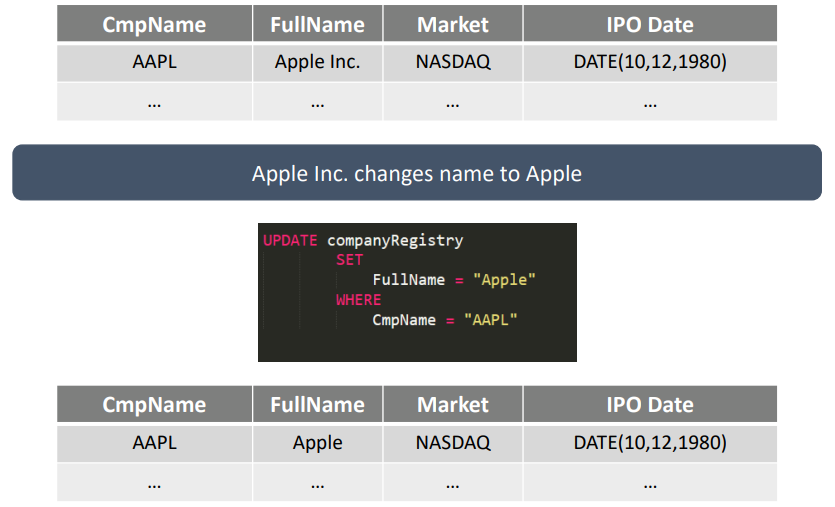
\includegraphics[scale=0.5]{29-data-source-registry-data-3}
\end{center}

\begin{center}
\textbf{Change Data Capture (CDC) is a set of design patterns used to determine (and track) the data that has changed so that action can be taken using the changed data.}
\end{center}

\subsection{Traditional Change Data Capture patterns}

\begin{center}
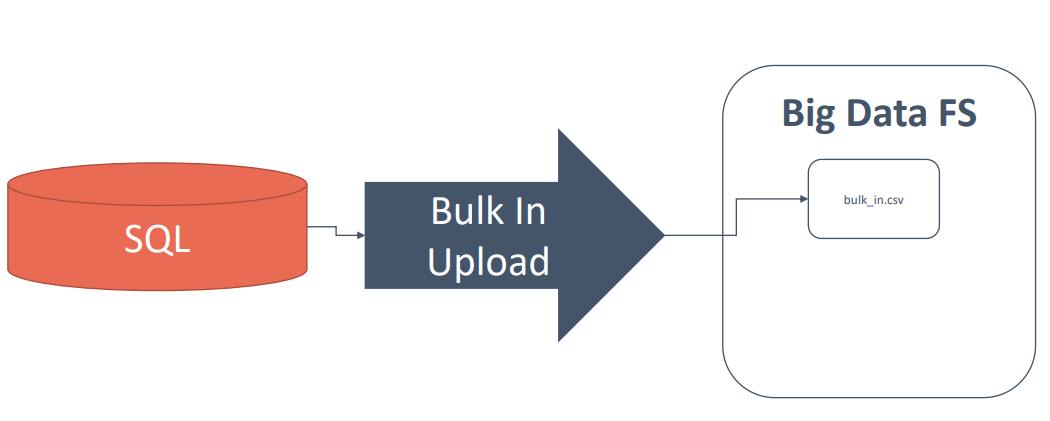
\includegraphics[scale=0.3]{30-traditional-change-data-capture-patterns-1}
\end{center}

\begin{center}
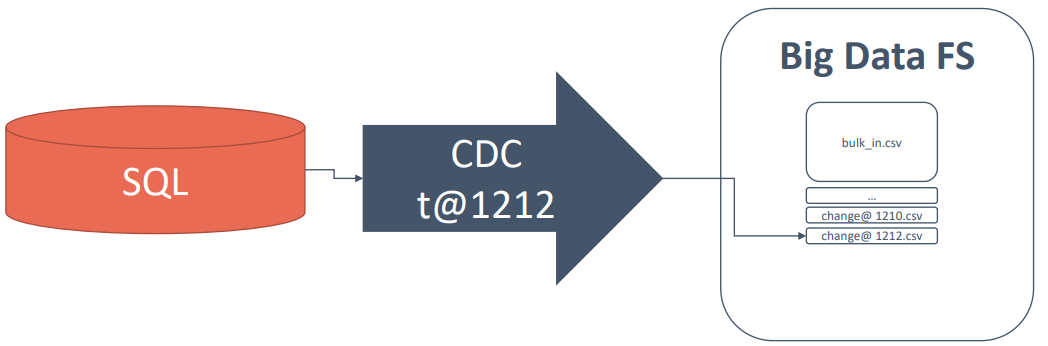
\includegraphics[scale=0.3]{31-traditional-change-data-capture-patterns-2}
\end{center}

\textbf{Invasive Database-side}
\begin{itemize}
	\item Timestamp on rows
	\item Version numebrs on rows based
	\item Status indicaters on rows
	\item Trigger on tables
\end{itemize}

\subsubsection{Invasive Database-side – Timestamps on rows}

When a change happens, the timestamp of when it happened is added as “Last Update” value.

\begin{center}
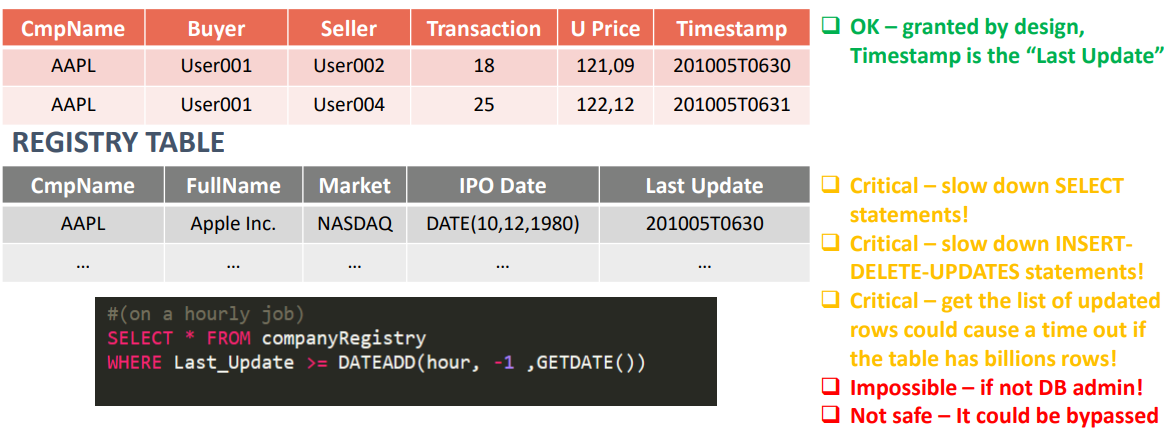
\includegraphics[scale=0.3]{32-invasive-database-side-version-numbers-on-rows}
\end{center}

\subsubsection{Invasive Database-side – Version numbers on rows}

When a change happens, a version+1 values is added to the fresh columns: all data with the latest version number is considered to have changed

\begin{center}
\includegraphics[scale=0.3]{33-invasive-database-side-version-number-on-rows}
\end{center}

\subsubsection{Invasive Database-side – Status Indicator}

A Boolean status is used to 

\begin{center}
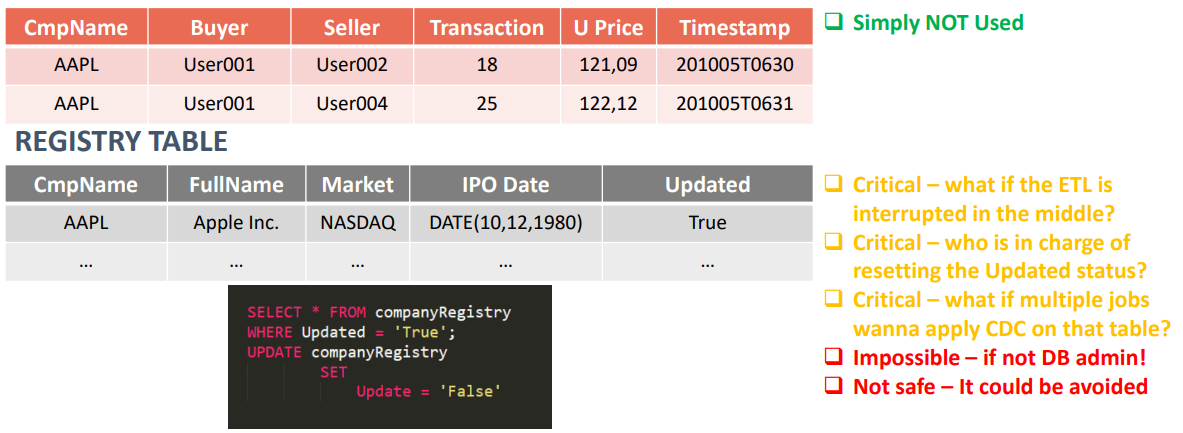
\includegraphics[scale=0.3]{34-invasive-database-side-status-indicator}
\end{center}

\subsubsection{Invasive Database-side – Triggers on Table}

A trigger is created after any write on the table

\begin{center}
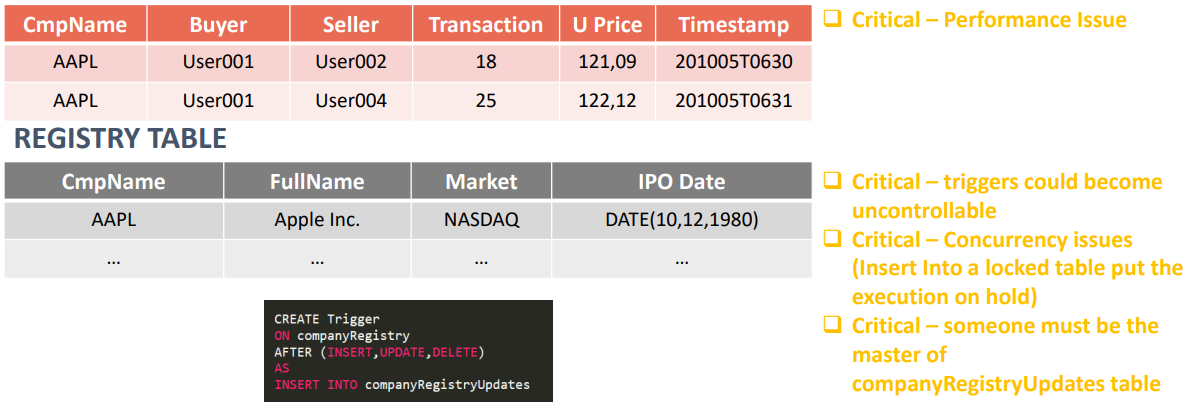
\includegraphics[scale=0.3]{35-invasive-database-side-triggers-on-table}
\end{center}

\subsubsection{Traditional Change Data Capture patterns}

\textbf{Invasive Application-side}

\begin{itemize}
	\item Event programming
	Give to the application the responsibility to propagate changes. Each time it commits something, the same operation must be sent also to the CDC system
\end{itemize}

\textbf{Invasive Database CPU-side}

\begin{itemize}
	\item Transaction log scanners
	Read and process some Database technical logs (i.e., transaction logs) to imply changes and to propagate them on CDC system
	\item Log Shipping
	Use an automatic DB backup process to propagate changes. This tool is mainly used as a Disaster Recovery solution.
\end{itemize}

\subsection{The Challenge - Can we design a CDC approach that…}

\subsubsection{CDC on Log Tables}

\begin{center}
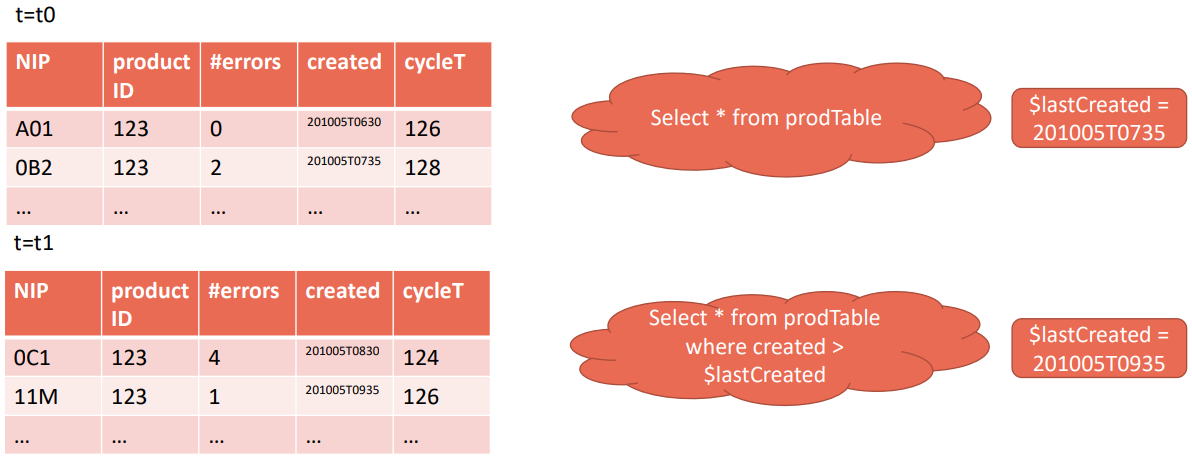
\includegraphics[scale=0.3]{36-cdc-on-log-tables}
\end{center}

\subsubsection{CDC on Registry Tables}

\begin{center}
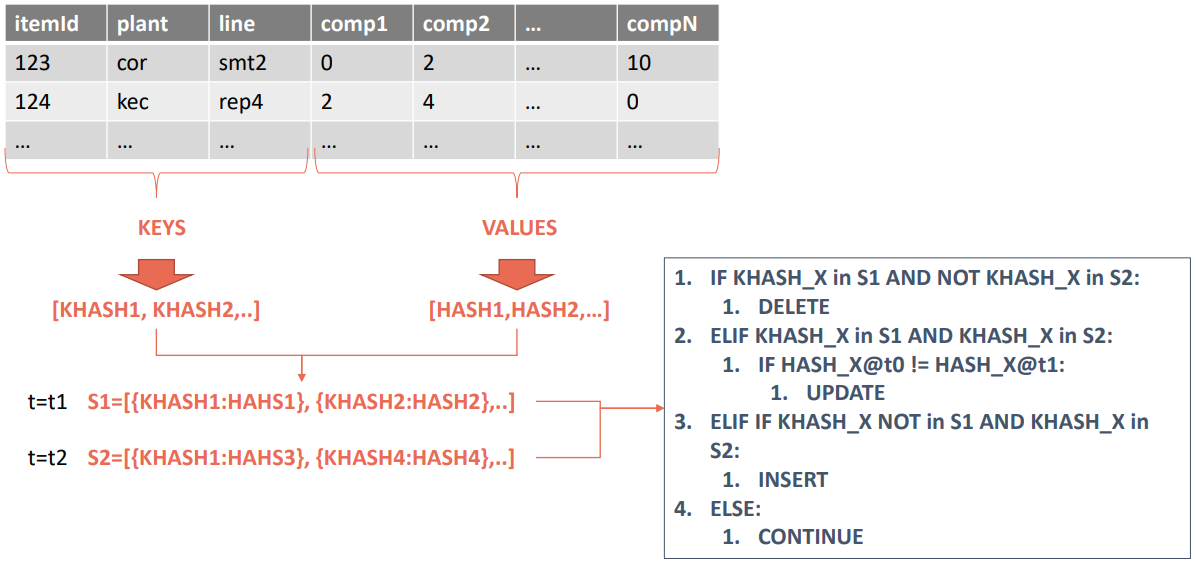
\includegraphics[scale=0.3]{37-cdc-on-registry-tables-1}
\end{center}

\hrulefill

\begin{center}
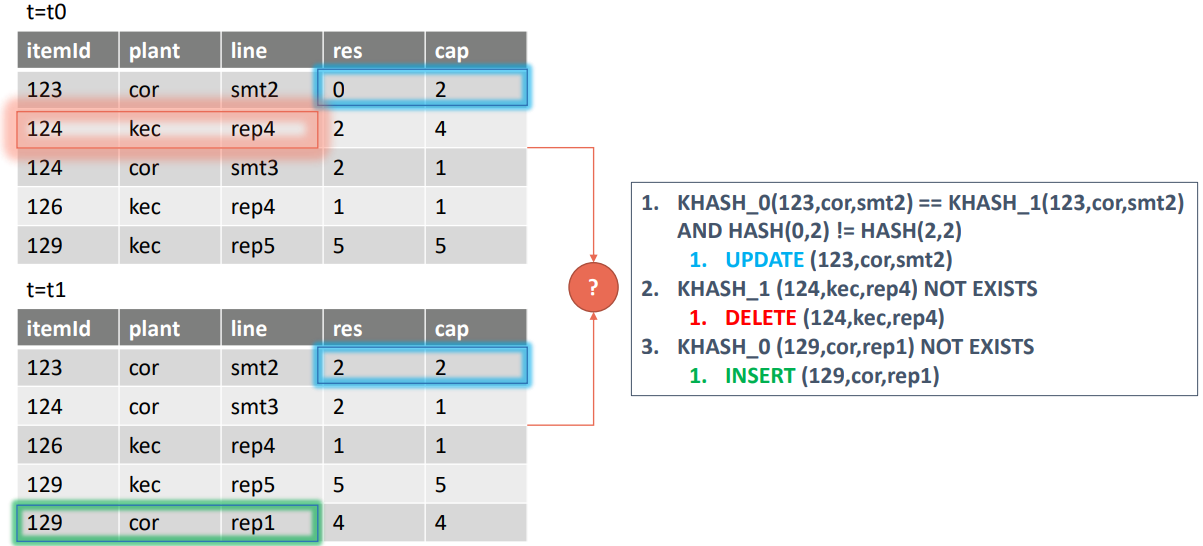
\includegraphics[scale=0.3]{38-cdc-on-registry-tables-2}
\end{center}

\subsubsection{The Diff \& Where CDC}

\begin{center}
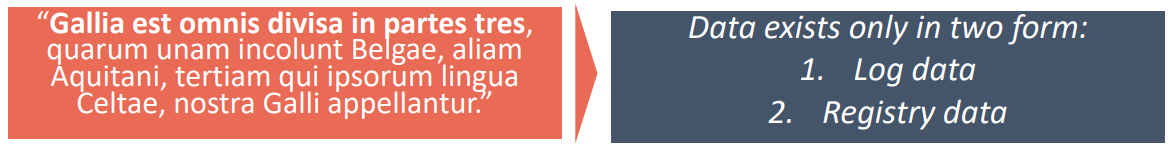
\includegraphics[scale=0.3]{39-the-diff-and-where-cdc}
\end{center}

\begin{itemize}
	\item Incremental extraction is one of the toughest task for any ETL system: the Diff \& Where incremental pattern could be used to solve this challenge
	\item Data can be found only in two shapes:
		- Log: any kind of data where there is the idea of chronosequence
		- Registry: any kind of data where there isn’t the idea of chrono-sequence
	\item The Diff \& Where incremental pattern is based on:
		- A "where-like" strategy to deal with loglike sources
		- A "diff-like" strategy to deal with registrylike sources
\end{itemize}

This way all the traditional pattern problems are easily solved

\subsubsection{The Diff \& Where CDC Bulk In}

\begin{center}
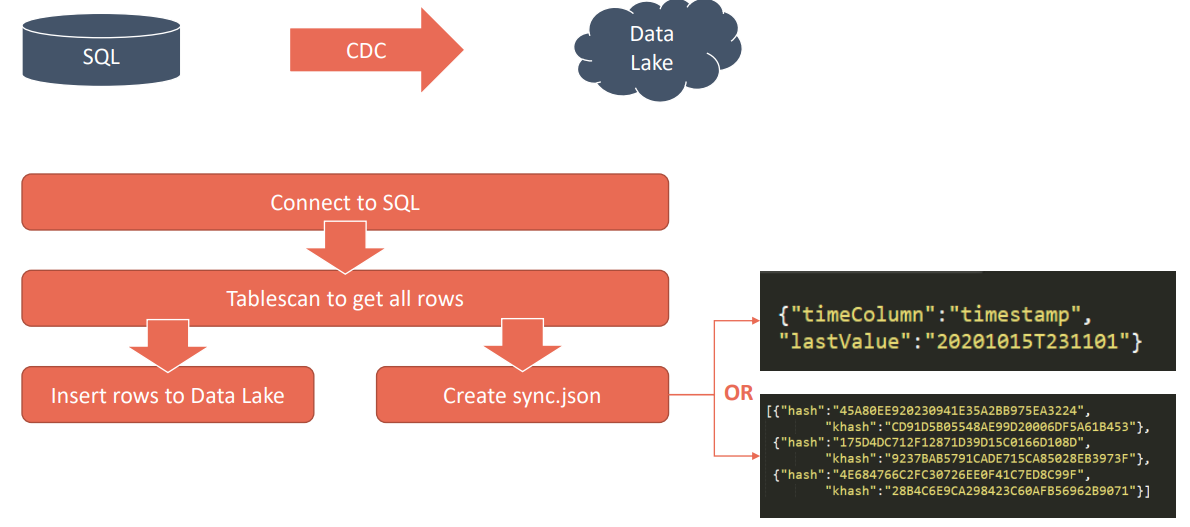
\includegraphics[scale=0.3]{40-the-diff-and-where-cdc-bulk-in}
\end{center}

\subsubsection{The Diff \& Where CDC Incremental}

\begin{center}
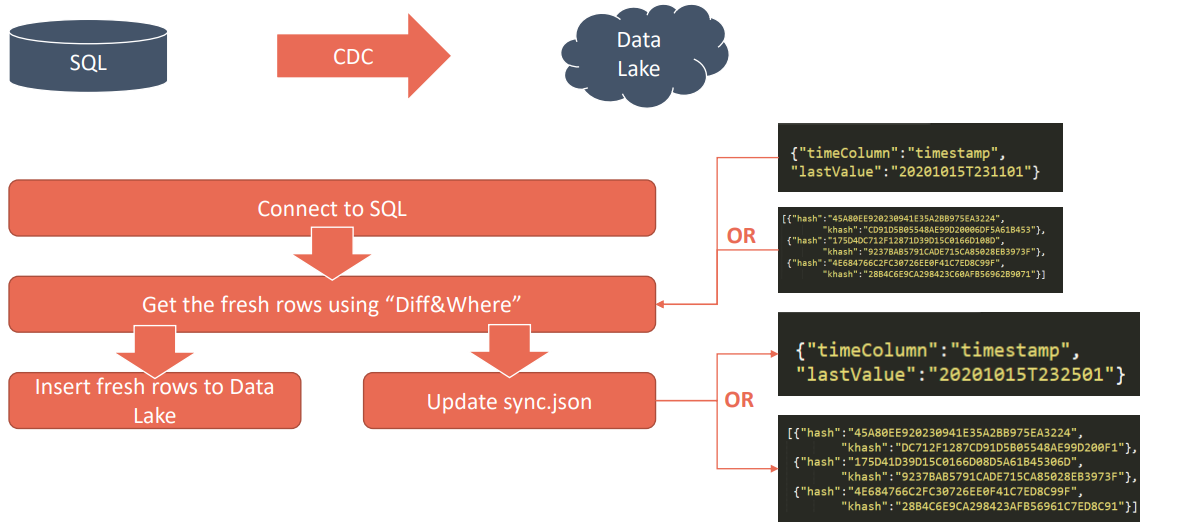
\includegraphics[scale=0.3]{41-the-diff-and-where-cdc-ncremental}
\end{center}

\subsubsection{The Diff \& Where Incremental could fail…}

\begin{center}
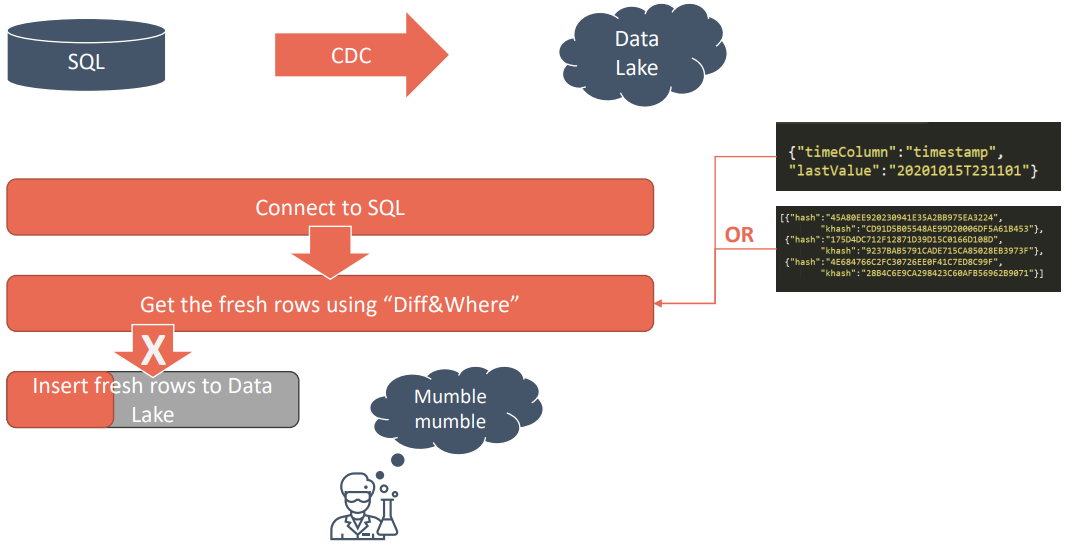
\includegraphics[scale=0.3]{42-the-diff-and-where-cdc-ncremental-could-fail}
\end{center}

\begin{center}
CDC Stateful? Or Stateless?

CDC should be Stateful? Or should be Stateless?

CDC could be transactional?

Is it possible to rollback a CDC target system

if the CDC process fail?
\end{center}

\subsubsection{CDC write transactionality – Example with file transfer}

\begin{center}
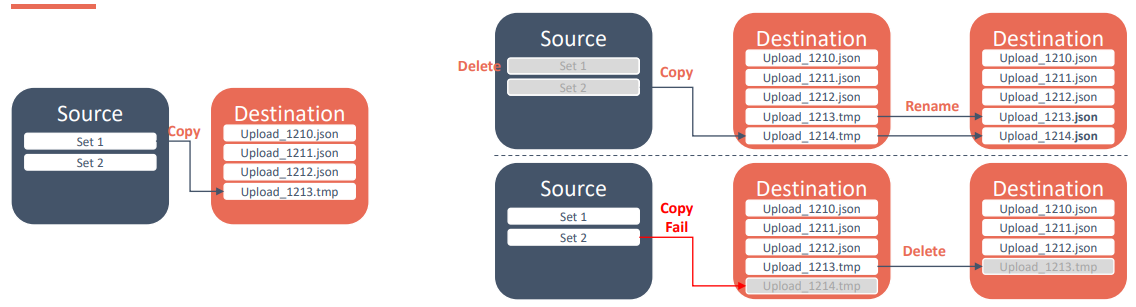
\includegraphics[scale=0.3]{43-cdc-write-transactionality-example-with-file-transfer}
\end{center}

\subsubsection{CDC write transactionality – Example with SQL}

\begin{center}
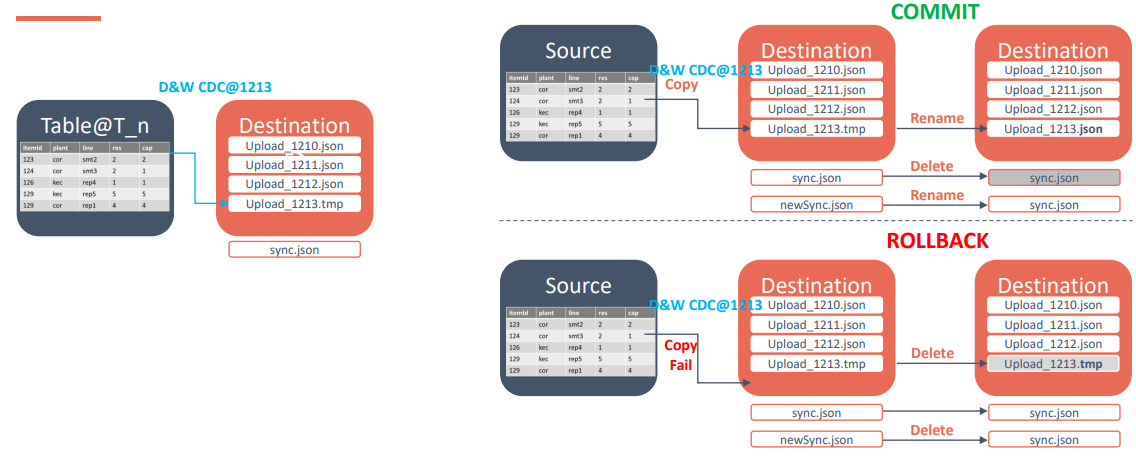
\includegraphics[scale=0.3]{44-cdc-write-transactionality-example-with-sql}
\end{center}

\subsubsection{CDC write transactionality}

\begin{center}
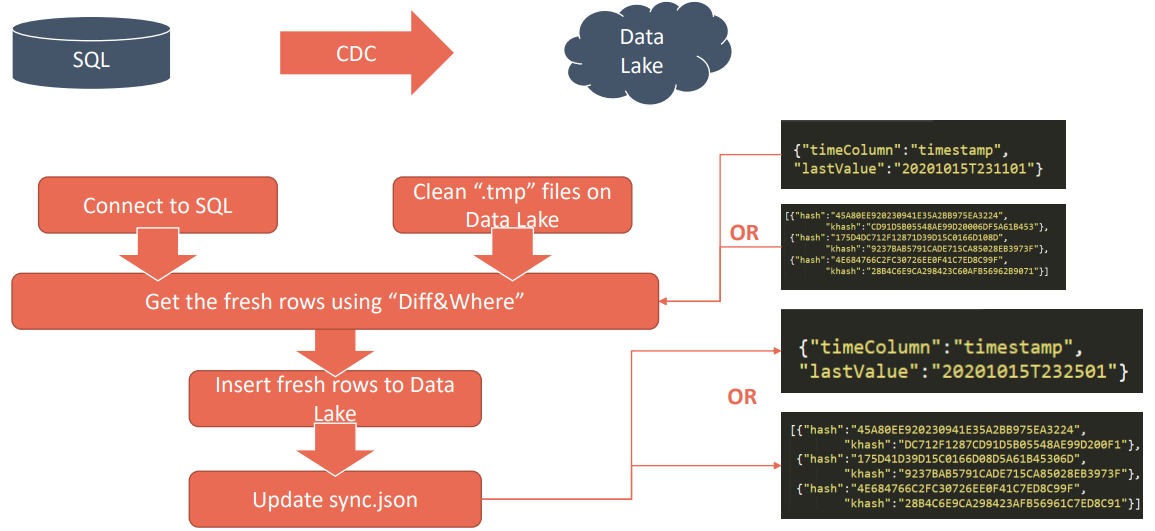
\includegraphics[scale=0.3]{45-cdc-write-transactionality}
\end{center}

\subsubsection{The Move and Rename Pattern}

\begin{center}
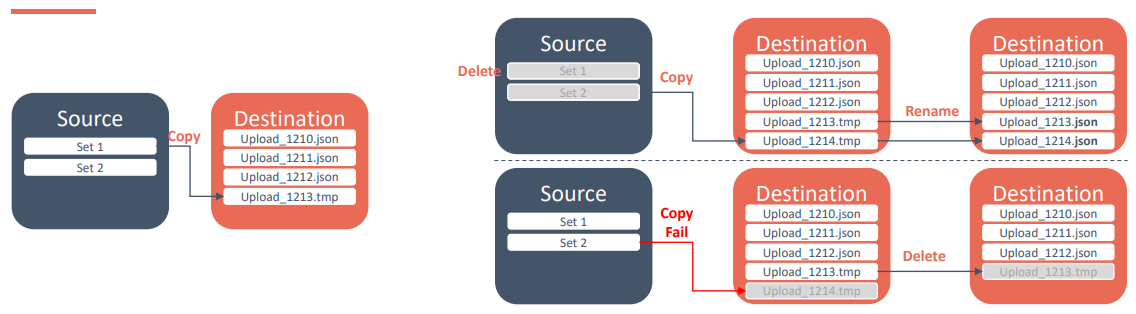
\includegraphics[scale=0.3]{46-the-move-and-rename-pattern}
\end{center}

\begin{itemize}
	\item Move and Rename is a very reliable way can be used when you need to move data from a source to a destination
	\item If the transfer time is long, different failures could happen (e.g., network interruption)
	\item While transferring requires time, renaming is an atomic operation
	\item Store and Forward makes the rollbacks policy easier to be implemented
	\item Move and Rename strategy is based on:
		- Using temporary filename to automatically tag file just wrote
		- Renaming every moved file at once at the end of the writing process
		- A clear final step to be executed at the beginning of any job as an automatic rollback 
\end{itemize}

\subsubsection{Panta Rei}

\begin{center}
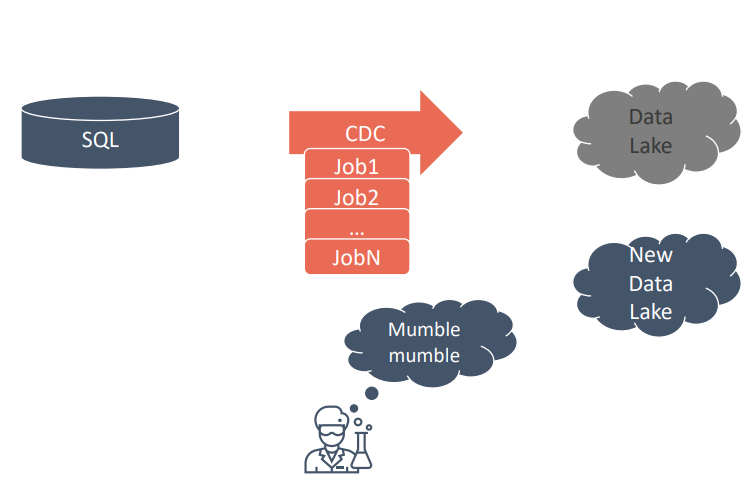
\includegraphics[scale=0.3]{47-punta-rei}
\end{center}

\textbf{And what if tomorrow I’ll change Data Lake provide?}

\subsubsection{The Adapter Pattern (Wrapper)}

\begin{center}
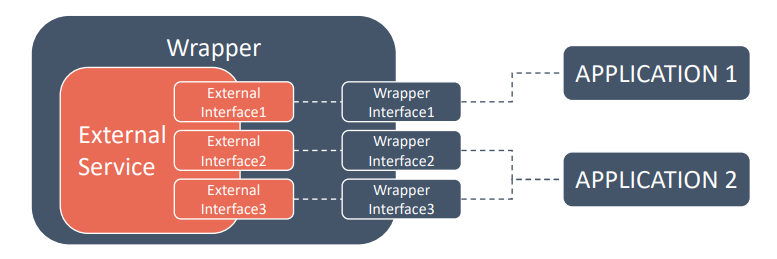
\includegraphics[scale=0.5]{48-the-adapter-pattern-1}
\end{center}

\begin{itemize}
	\item Service Adapter Pattern allows the interface of an existing class to be used as  another interface
	\item Service Adapter Pattern is the most reliable way to call external services
	\item The Wrapper Class exposes the External Services interfaces
	\item Internal Services cannot access external Services directly
	\item Wrapping External Services reduces the lock-in effect
	\item Centralizing all the calls to External Services allows users to implement once tracing strategies
\end{itemize}

\begin{center}
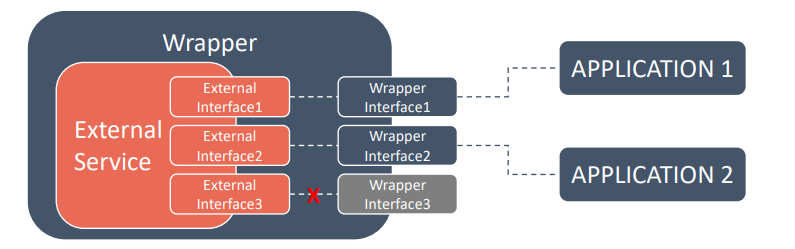
\includegraphics[scale=0.5]{49-the-adapter-pattern-2}
\end{center}

\begin{itemize}
	\item The wrapper can also hide some methods to avoid application use them!
\end{itemize}

\subsubsection{Finally Data Scientist time has come}

\begin{center}
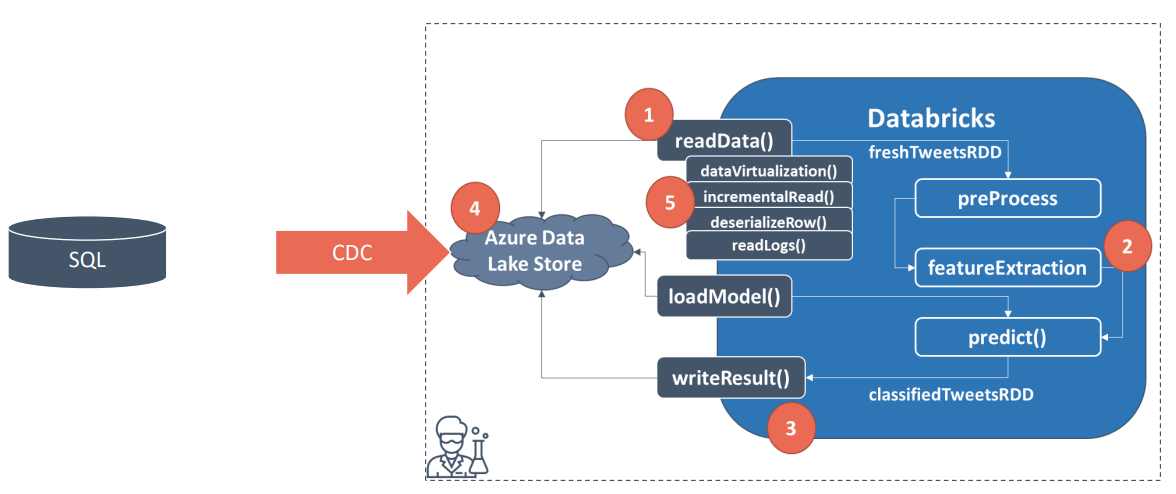
\includegraphics[scale=0.3]{50-finally-data-scientist-time-has-come}
\end{center}